\chapter{Wellen in einem Kanal\label{chapter:wellen}}
\lhead{Wellen in einem Kanal}
\begin{refsection}
\chapterauthor{Daniela Meier und Hansruedi Patzen}

\begin{equation}
	y'' + (ax^2+bx+c)y = 0
	\label{wellen:grundgleichung}
\end{equation}

Dieses Kapitel besch"aftigt sich mit Ausbreitung von Wellen in einem 
parabolischen Kanal. Die Ausbreitung wird mittels Analyse der Wellengleichung 
n"aher betrachtet.

%
% einleitung.tex -- Einleitung zum Skript ueber Differentialgleichungen
%
% (c) 2015 Prof Dr Andreas Mueller, Hochschule Rapperswil
%
\chapter{Einleitung\label{chapter:einleitung}}
\lhead{Einleitung}
\rhead{}
In XKCD 135 (Abbildung~\ref{einleitung:xkcd135})
beschreibt Randall Munroe erdachte Aufgaben "uber die
Jagdgewohnheiten von Velociraptoren, Fragen, bei denen es um Leben
und Tod geht.
Die Aufgaben k"onnen zwar ohne Differentialgleichungen gel"ost
werden, aber sie k"onnen leicht zu noch spannenderen Aufgaben
verallgemeinert werden, die nicht ohne die Kenntnisse von 
Differentialgleichungen gel"ost werden k"onnen.
Dies zeigt, dass die Kenntnis der L"osungsverfahren von Differentialgleichungen
eine Frage von Leben und Tod ist.

\index{Newton!Isaac}
Isaac Newtons Grundgesetze der Dynamik sind die ersten Beispiele
von Differentialgleichungen.
Sein erstes Gesetz besagt:
\begin{quote}
\em
Ein K"orper verharrt im Zustand der Ruhe oder der gleichf"ormigen Translation,
sofern er nicht durch einwirkende Kr"afte zur "Anderung seines Zustands
gezwungen wird.
\end{quote}
In der Abwesenheit von Kr"aften ver"andert sich die Geschwindigkeit nicht,
oder 
\[
\frac{d}{dt}\vec{v}=0,
\]
wobei $\vec{v}$ der Vektor der Geschwindigkeit ist.
Das erste Gesetz oder Tr"agheitsprinzip wurde schon von Galileo Galilei
formuliert.
\index{Tragheitsprinzip@Tr\"agheitsprinzip}

\begin{figure}
\centering
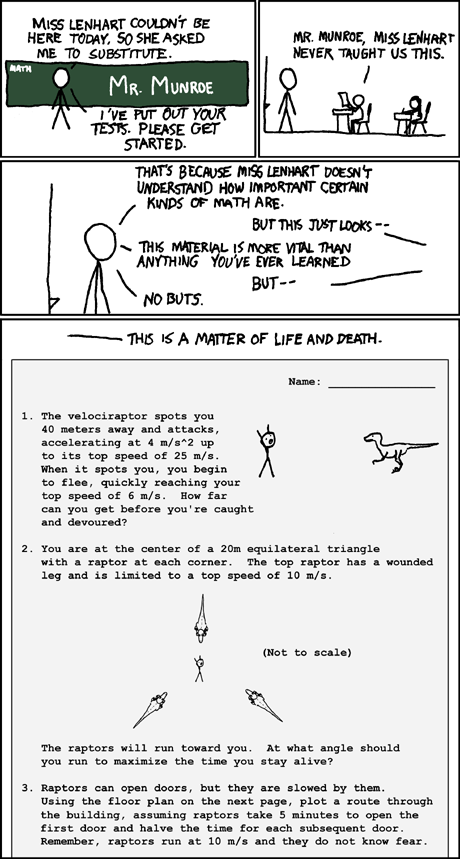
\includegraphics[width=0.7\hsize]{chapters/substitute.png}
\caption{xkcd 135 mit von Randall Munroe erdachten Aufgaben "uber die
Jagdgewohnheiten von Velociraptoren.
\label{einleitung:xkcd135}}
\end{figure}%


Das zweite Gesetz besagt:
\begin{quote}
\em
Die "Anderung der Bewegung ist der Einwirkung der bewegenden Kraft
proportional und geschieht nach der Richtung derjenigen geraden Linie,
nach welcher jene Kraft wirkt.
\end{quote}
Mit {\em Bewegung}
meint Newton den Impuls $\vec{p}=m\vec{v}$,
\index{Impuls}
das zweite Gesetz wird in moderner Schreibweise
\[
\frac{d}{dt}(m\vec{v}) = \vec{F}.
\]
In beiden F"allen wird die "Anderung einer Zustandsvariablen, n"amlich
des Impulses, mit dem aktuellen Zustand, typischerweise der Position,
verkn"upft.
Die Newtonsch-Bewegungsgesetze sind Differentialgleichungen.
\index{Newton!Bewegungsgesetz}

Das neue Werkzeug der Infinitesimalrechnung bescherte der exakten
Naturwissenschaft eine F"ulle neuer Probleml"osungen, die alle
nach dem gleichen Prinzip vorgingen.
Finde die Differentialgleichungen zwischen den Zustandsvariablen
eines Systems, "ublicherweise durch Anwendung des zweiten
Newtonschen Gesetztes, l"ose die Differentialgleichungen und
ziehe die Schl"usse.
Es zeigte sich jedoch bald, dass viele Differentialgleichungen
keine L"osungen haben, die sich mit den bisher bekannten Funktionen
ausdr"ucken lassen.
Man behalf sich kurzerhand damit, neue Funktionen zu definieren, 
die bald Anwendungen in den verschieden Gebieten der Technik fanden.
Die Bessel-Funktionen sind mittlerweile so wichtig, dass sie in keiner
Computer-Bibliothek f"ur mathematische Funktionen fehlen d"urfen.
\index{Bessel-Funktion}

Die Herkunft der Kr"afte wird in den Newtonschen Gesetzen nicht weiter
gekl"art, doch Newton selbst beschreibt mit seinem Gravitationsgesetz
die Herkunft der Kr"afte, die die Planeten im Sonnensystem auf ihren Bahnen
halten.
\index{Kepler!Johannes}
\index{Kepler-Bahn}
Er zeigt, dass die Keplerschen Ellipsenbahnen L"osungen seiner
Bewegungsgleichungen sind.
Die rein kinematische Beschreibung durch Kepler machte einem
dynamischen Verst"andnis Platz, welches nun auch die gegenseitigen
Einfl"usse der Planeten aufeinander zu berechnen gestattet.
Und tats"achlich war Newton der erste, der sich dar"uber Gedanken
machte, wie sich das Sonnensystem "uber lange Zeit entwickeln wird.
Seine Schlussfolgerung aus seinen aus heutiger Sicht rudiment"aren
Untersuchungen: das Sonnensystem ist instabil, "uber die Jahrmillionen 
werden die Planeten in den interstellaren Raum geschleudert werden.

Die industrielle Revolution brachte eine Vielzahl von Maschinen,
\index{industrielle Revolution}
die automatisch geregelt werden mussten.
Ingenieure entwickelten eine ganze Reihe von einfallsreichen L"osungen,
doch erst in der Mitte des 19.~Jahrhunderts konnten Physiker diese
Apparaturen mit Differentialgleichungen erkl"aren und ihre Stabilit"at
untersuchen.
Im zwanzigsten Jahrhundert reiften die mathematischen Hilfsmittel
soweit, dass auch instabile L"osungen untersucht werden konnten,
wie sie bei nichtlinearen Differentialgleichungen auftreten.
Mittlerweile ist das Auftreten Instabilit"aten recht gut verstanden
und klassifiziert. 
Die Technik der Linearisierung erm"oglicht zum Beispiel die
Hopf-Bifurkation zu verstehen.
\index{Hopf-Bifurkation}
\index{Bifurkation!Hopf}
Auch die Sattel-Knoten-Bifurkation und die Heugabel-Bifurkation
lassen sich in Anwendungen finden.
\index{Bifurkation!Sattel-Knoten-}
\index{Sattel-Knoten-Bifurkation}
\index{Bifurkation!Heugabel-}
\index{Heugabel-Bifurkation}
Und die Chaos-Theorie versteht sogar, wie "uber eine Kaskade von
Bifurkationen die Bewegung eines Systems jede Vorhersagbarkeit verliert,
es bewegt sich chaotisch.
\index{Chaos}

In vielen F"allen l"asst sich eine Differentialgleichung erst dann
verstehen, wenn man in komplexen Zahlen arbeiten. 
Die Hopf-Bifurkation tritt zum Beispiel genau dann auf, wenn eine
Bedingung "uber die Eigenwerte des linearisierten Systems erf"ullt ist.

Weitere Literaturhinweise im Literaturverzeichnis auf
Seite~\pageref{skript:literatur}.



\section{Herleitung Ausgangsformel}
Gem"ass \cite{wellen:smirnow2}, lautet die allgemeine Differentialgleichung der 
Welle:

\begin{equation*}
	\frac{\partial^2 u}{\partial t^2}
	=
	c^2
	\left(
		\frac{\partial^2 u}{\partial x^2} 
		+ \frac{\partial^2 u}{\partial y^2} 
		+ \frac{\partial^2 u}{\partial z^2}
	\right)
	\label{eq:wellen:allgemeineDGL}
\end{equation*}

Da es sich in der ausgew"ahlten Problemstellung nur eine zweidimensionale Welle 
handelt, fallen die y- und z-Koordinate weg. Die Gleichung vereinfacht sich 
dadurch zu:

\begin{equation}
	\frac{\partial^2 u}{\partial t^2}
	=
	c^2
	\left(
		\frac{\partial^2 u}{\partial x^2} 
	\right)
	\label{eq:wellen:allgemeineDGLvereinfacht}
\end{equation}

Zur L"osung der vereinfachten Wellengleichung 
\ref{eq:wellen:allgemeineDGLvereinfacht} wird nun die Theorie des 
Separationsansatzes angewendet. Gem"ass dieser kann die von der Zeit $t$ und 
der Ortskoordinate $x$ abh"angigen Funktion $u(x,t)$ in ein Produkt 
zweier Funktionen $X(x)$ und $T(t)$ umgewandelt werden.

\begin{equation}
	u (x,t) = X(x) T(t)
	\label{eq:wellen:separierteFunktion}
\end{equation}

Ausgehend von der Gleichung \ref{eq:wellen:allgemeineDGLvereinfacht} wird die 
Funktion \ref{eq:wellen:separierteFunktion} auf der linken Seite zweimal 
partiell nach $t$ und auf der rechten Seite zweimal partiell nach $x$ 
abgeleitet:

\begin{equation*}
	T''(t) X(x) = c^2 X''(x)T(t)
\end{equation*}

Nach einer Division durch $T(x)X(x)$ sind die Variablen separiert. Der neu 
entstandene Term kann nur dann funktionieren, wenn beide Seiten der Gleichung 
konstant sind.

\begin{equation*}
	\frac{T''(t)}{T(t)}
	=
	c^2 \frac{X''(x)}{X(x)} = \text{konstant} = \lambda
\end{equation*}

Es folgen nun also zwei l"osbare Differentialgleichungen zweiter Ordnung:

\begin{align*}
	T'' &= \lambda T(t) \\
	X'' &= \frac{\lambda}{c^2}X(x).
\end{align*}

Bei der betrachteten Problemstellung, wird davon ausgegangen, dass die 
Zeit konstant ist. Aus diesem Grund wird ab hier nur noch auf die Gleichung 
der Funktion $X(x)$ weiter eingegangen.

Die Gleichung

\begin{equation*}
	X''(x) - \frac{\lambda}{c^2} X(x) = 0
\end{equation*}
widerspiegelt die Wellengleichung, die in der Fortsetzung betrachtet wird.

Mit dem Faktor $\frac{\lambda}{c^2}$ k"onnen verschiedene 
Geschwindigkeitsprofile betrachtet werden. Hier wird unter anderem auf den 
speziellen Fall eines parabolischen Profils eingegangen. Die zu untersuchende 
Differentialgleichung ergibt sich hiermit zu der am Anfang definierten 
Gleichung \ref{eq:wellen:grundgleichung}, mit den frei w"ahlbaren Variablen 
${a,b,c} \in \mathbb{R}$, sowie den Anfangsbedingungen $y(0) = a_0$ und $y'(0) 
= a_1$.


\section{Potenzreihenl"osung}
Als L"osungsansatz wird der im Kapitel \ref{chapter:potenzreihen} 
kennengelernte Potenzreihenansatz verwendet.

Zuerst wird die Potenzreihe f"ur $y(x)$ aufgestellt und zweimal abgeleitet.

\begin{align}
	y(x)
	&=
	\sum_{k = 0}^{\infty} a_{k}x^k
	=
	a_0 + a_1x + a_2x^2 + a_3x^3 + a_4x^4 + a_5x^5 + a_6x^6 + \dotsb
	\label{eq:wellen:nullteableitung}
	\\
	y'(x)
	&=
	\sum_{k=0}^{\infty} a_{k+1}(k+1)x^k
	=
	a_1 + 2a_2x + 3a_3x^2 + 4a_4x^3 + 5a_5x^4 + 6a_6x^5+ \dotsb
	\label{eq:wellen:ersteableitung}
	\\
	y''(x)
	&=
	\sum_{k = 0}^{\infty} a_{k+2}(k+1)(k+2)x^k
	=
	2a_2 + 3 \mathbin{\cdot} 2a_3x + 4 \mathbin{\cdot} 3a_4x^2 + 5 
	\mathbin{\cdot} 4a_5x^3 + 6 \mathbin{\cdot} 5a_6x^4 + \dotsb
	\label{eq:wellen:zweiteableitung}
\end{align}

Aus den beiden Gleichungen \ref{eq:wellen:nullteableitung} und
\ref{eq:wellen:zweiteableitung} und dem Umstellen der Anfangsgleichung in die 
Form
\begin{equation*}
	y'' = -(ax^2+bx+c)y
\end{equation*}
kann nun der Koeffizientenvergleich erstellt werden. 

Statt die Koeffizienten einfach reihenweise aufzustellen, wird der Vergleich 
mit Hilfe einer Tabelle gemacht.

\begin{equation}
	\begin{array}{r c r | c r | c r | c r c}
	y(x) & = &
	a_0 & + & a_1x & + & a_2x^2 & + \dotsb
	\\
	\hline&&&&&&&\\[-2ex]
	y''(x) & = &
	2\cdot1 a_2 & + & 3\cdot2 a_3x & + & 4\cdot3 a_4x^2 & + \dotsb
	\\
	& = &
	& & & + &- aa_0x^2 & + \dotsb
	\\
	& &
	& &- ba_0x & + &- ba_1x^2 & + \dotsb
	\\
	& &
	-ca_0 & + &- ca_1x & + &- ca_2x^2 & + \dotsb
	\\
	\hline&&&&&&&\\[-2ex]
	& &
	a_2 = -\frac{1}{2 \cdot 1}ca_0,
	& & a_3 = -\frac{1}{3 \cdot 2}(ba_0+c_a1),
	& & a_4 = -\frac{1}{4 \cdot 3}(aa_0+ba_1+ca_2),
	& \dots
	\end{array}
	\label{eq:wellen:koeffizietenvergleichtabelle}
\end{equation}

Die Verschiebung der verschiedenen $a_k$ in der Tabelle 
\ref{eq:wellen:koeffizietenvergleichtabelle} kann einfach erkl"art werden. 
Aufgrund der zweiten Ableitung werden die $a_k$ der zweiten Zeile um zwei nach 
links geschoben. Eine weitere Verschiebung gibt es wegen des Polynomgrades.

Da die $a$-Summanden mindestens die Form $ax^2$ haben, verschiebt sich die 
dritte Zeile um zwei nach rechts. Die $b$-Summanden haben mindestens Die Form 
$bx^1$, daher die Verschiebung der vierten Zeile um eins nach rechts. Einzig 
die f"unfte Zeile mit den $c$ wird nicht verschoben, da es mindestens als 
$cx^0$ vorhanden ist. Somit lassen sich die jeweiligen $a_k$ und ihre 
Abh"angigkeiten direkt aus den jeweiligen Spalten ablesen.

Aus den in der Tabelle berechneten $a_k$ l"asst sich nun eine allgemeine 
Rekursionsformel

\begin{equation*}
	\begin{split}
		a_{k+2} &= -\frac{1}{(k+2)(k+1)} (aa_{k-2}+ba_{k-1}+ca_k) \\
		\Leftrightarrow \qquad
		a_k &= -\frac{1}{k(k-1)} (aa_{k-4}+ba_{k-3}+ca_{k-2}), \qquad k \in 
		\mathbb{N} \setminus \{0, 1\}, a_{k<0} = 0
	\end{split}
\end{equation*}
herauslesen. 

Daraus kann nun die L"osungsgleichung
\begin{equation}
	y(x) = a_0 + a_1x 
	-\sum_{k=2}^{\infty}\frac{1}{k(k-1)}(aa_{k-4}+ba_{k-3}+ca_{k-2})x^k
	\label{eq:wellen:ygleichung}
\end{equation}
aufgestellt werden.


\section{Erkenntnisse bei der Variation von \texorpdfstring{$k_{max}$}{kmax}}

Es wird davon ausgegangen, dass sich mit der Variation von $k_{max}$ bei der 
Welle keine grossen Ver"anderungen einstellen. Die Werte werden immer ab einem 
gewissen Punkt ins Positive oder Negative explodieren, da das $x^k$ irgendwann 
dominiert. Mit $k_{max}$ wird die Anzahl der Summanden bezeichnet, die f"ur die 
Berechnung der Potenzreihe verwendet werden. 

\begin{equation*}
y(x) = a_0 + a_1x 
-\sum_{k=2}^{k_{max}}\frac{1}{k(k-1)}(aa_{k-4}+ba_{k-3}+ca_{k-2})x^k
\end{equation*}

Es werden die Startbedingungen gem"ass den Gleichungen 
\ref{wellen:Startbedingungen1} festgelegt.

\begin{equation}
	\begin{split}
		a_0 &= 1\\
		a_1 &= 0\\
		a &= 1\\
		b &= 0\\
		c &= -1
	\end{split}
	\label{wellen:Startbedingungen1}
\end{equation}

Auf folgenden Grafiken wird veranschaulicht, was mit der Welle passiert, wenn 
das $k_{max}$ jeweils um 30 vergr"ossert wird. Es wird dann "uberpr"uft, ob 
sich die Behauptung der kleinen Ver"anderungen als wahr herausstellt.

\begin{center}
	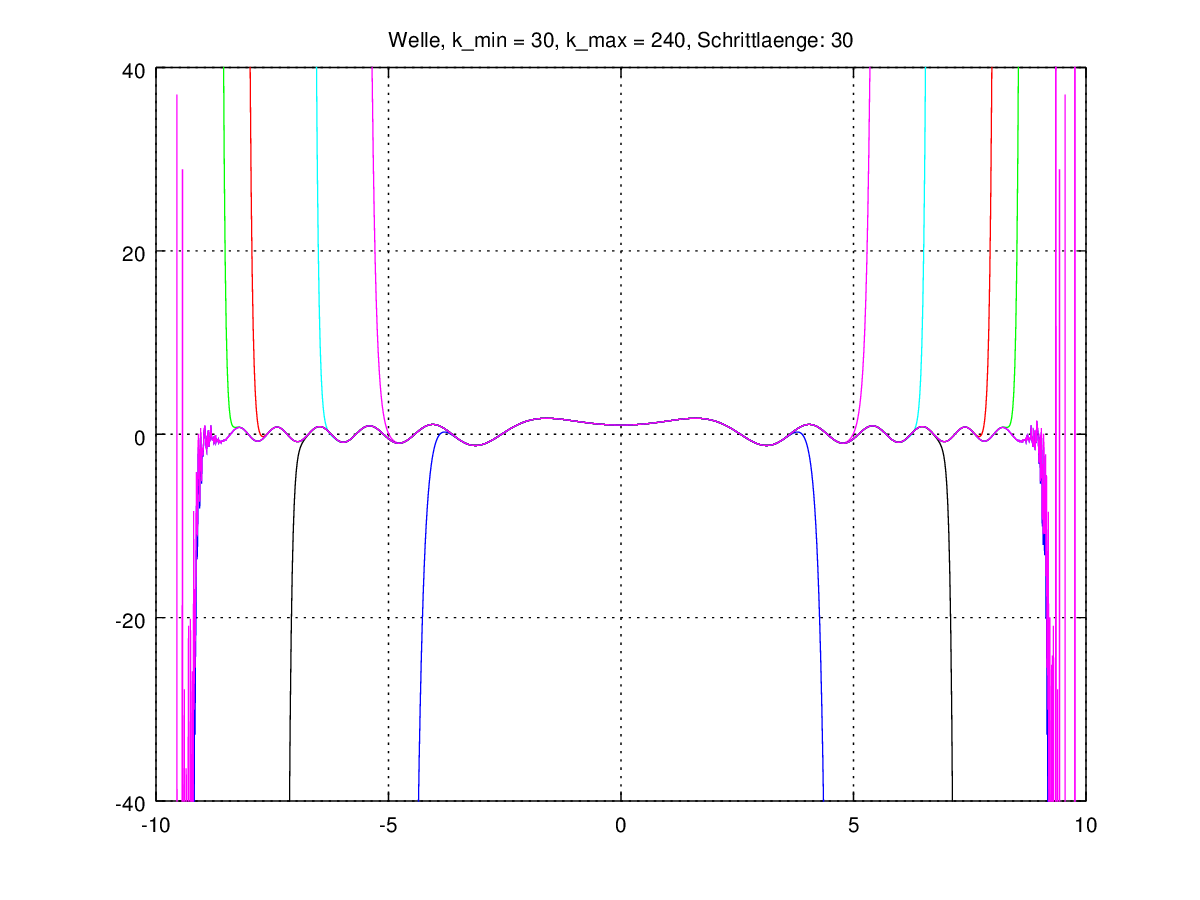
\includegraphics[scale=0.69]{./wellen/images/kmax/krangewaveeven.png}
\end{center}

Die Behauptung, dass der Wert irgendwann explodiert, ist, wie ersichtlich, 
wahr. Der Punkt wo die Werte gegen $\infty$ gehen verschiebt sich immer mehr 
nach rechts, zu gr"osseren $x$-Werten. Dies wird dadurch erkl"art, dass es 
immer l"anger geht, bis der $x^k$-Term dominiert. Je mehr der $k_{max}$-Wert 
gesteigert wird, umso besser wird die Approximation an die Welle. Ab einer 
gewissen Gr"osse von $k_{max}$ kann das Programm die Werte nicht mehr genau 
bestimmen, was die unregelm"assigen Ausschl"age erkl"art.

Aufgrund dieser Messungen wird $x$ f"ur die weiteren Berechnungen auf $x \in 
[-8;8]$ und $k_{max}$ auf 180 beschr"ankt, damit die $y$-Werte nicht 
explodieren und keine unkontrollierten Messwerte entstehen.

Mit den in diesem Kapitel festgelegten Startbedingungen und Einschr"ankungen 
ergibt dies folgende Grafik:
\begin{center}
	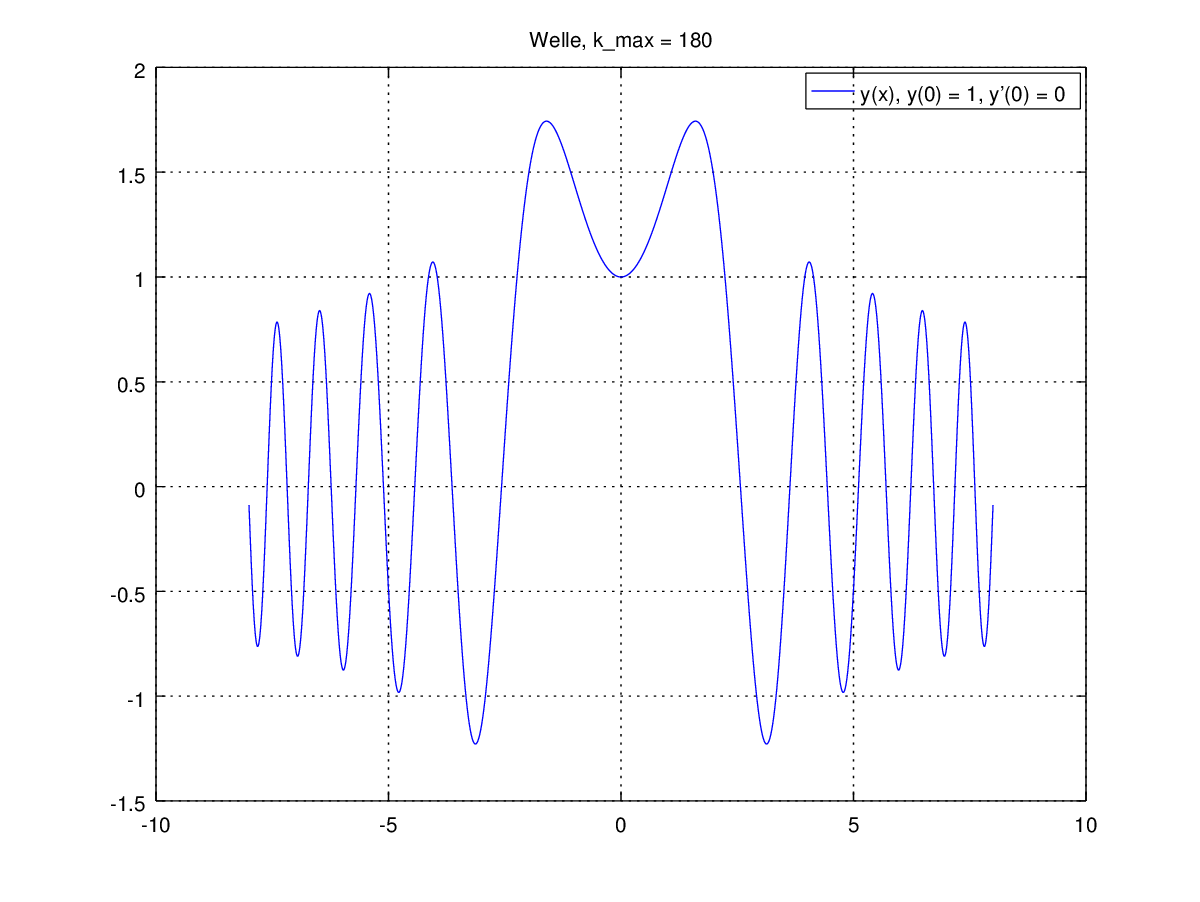
\includegraphics[scale=0.69]{./wellen/images/kmax/ak180-88wave.png}
\end{center}

\section{Erkenntnisse bei der Variation von \texorpdfstring{$a$}{a}, 
\texorpdfstring{$b$}{b} und \texorpdfstring{$c$}{c}}

Die Anfangsbedingungen $a_0$ und $a_1$ k"onnen beliebig festgelegt werden. Da 
sich die Wellen im betrachteten Fall um den Entwicklungspunkt $x_0=0$ bewegen, 
beschreibt das $a_0$ den y-Achsenabschnitt und das $a_1$ die Steigung im Punkt 
$y(0)$. Die gew"ahlten Werte von $a_0$ und $a_1$ sind jeweils in der Grafik 
ersichtlich.

\subsection{Eliminierung von $a$ und $b$}
\label{wellen:Eliminierungab}

Zu Beginn wird das vorgegebene, parabelf"ormige Geschwindigkeitsprofil 
n"aherungsweise in eine Konstante umgewandelt indem $a$ verschwindend klein 
gew"ahlt wird und $b$ gleich $0$ gesetzt wird. Die beiden Variablen werden also 
eliminiert und folgende Differentialgleichung wird betrachtet:

\begin{equation}
	y''+ cy = 0.
	\label{wellen:lineareDGL}
\end{equation}


F"ur positive Werte von c kann die L"osung dieser Gleichung 
\ref{wellen:lineareDGL} mit dem charakteristischen Polynom bestimmt werden. 
Die L"osungen des charakteristischen Polynoms

\begin{equation}
	p(\lambda) = [(\lambda+\mu)^2+\omega^2] =0
	\label{wellen:charakteristischesPolynom}
\end{equation}

sind

\begin{equation}
	\begin{split}
	y_1 &= C_1e^{-\mu x}\cos(\omega x) \\
	y_1 &= C_2e^{-\mu x}\sin(\omega x).
	\end{split}
	\label{wellen:lsgcharakteristischesPolynom}
\end{equation}

Das zur Gleichung \ref{wellen:lineareDGL} geh"orende charakteristische Polynom 
ist gem"ass \ref{wellen:charakteristischesPolynom}

\begin{equation*}
	p(\lambda) = [\lambda^2 + c] =0.
\end{equation*}

Somit folgt die allgemeine L"osung der Differentialgleichung 
\ref{wellen:lineareDGL} gem"ass \ref{wellen:lsgcharakteristischesPolynom}

\begin{equation}
	y(x) = C_1 \cos(\sqrt{c}x) + C_2 \sin(\sqrt{c}x)
	\label{wellen:LsglineareDGL}
\end{equation}

Um die Konstanten $C_1$ und $C_2$ zu bestimmen m"ussen die Anfangsbedingungen 
$a_0$ und $a_1$ bekannt sein. Um die Abh"angigkeit aufzuzeigen, muss zuerst die 
erste Ableitung der L"osung \ref{wellen:LsglineareDGL} aufgestellt werden.

\begin{equation}
	y'(x)=-C_1 \sqrt{c} \sin(\sqrt{c}x) + C_2 \sqrt{c} \cos(\sqrt{c}x)
\end{equation}

Der Wert bei $y(0)$ ist definiert als $a_0$ und die Steigung am Punkt $y'(0)$ 
ist das $a_1$. Setzt man $x=0$ in die L"osungsgleichung 
\ref{wellen:LsglineareDGL} ein, k"onnen $C_1$ und $C_2$ bestimmt werden.

\begin{equation}
	\begin{split}
		y(0) = C_1 = a_0 &\Leftrightarrow C_1 = a_0 \\
		y'(0) = C_2 \sqrt{c} = a_1 &\Leftrightarrow C_2 = \frac{a_1}{\sqrt{c}}
	\end{split}
	\label{wellen:KonstantenC1C2}
\end{equation}

Setzt man diese Konstanten \ref{wellen:KonstantenC1C2} in die L"osungsgleichung 
\ref{wellen:LsglineareDGL} 
ein, ergibt sich die Gleichung, die sich mit den Startangaben, die definiert 
werden, f"ur positive $c$-Werte berechnen l"asst.

\begin{equation}
	y(x) = a_0 \cos(\sqrt{c}x) + \frac{a_1}{\sqrt{c}} \sin(\sqrt{c}x)
	\label{wellen:LSGleichung}
\end{equation}

In den folgenden zwei Grafiken werden die zwei Grundfunktionen von ``reinem''
Sinus (erste Grafik) und Cosinus (zweite Grafik) aufgezeigt. Daf"ur muss 
entweder $a_0$ oder $a_1$ gleich Null gesetzt werden.

\noindent
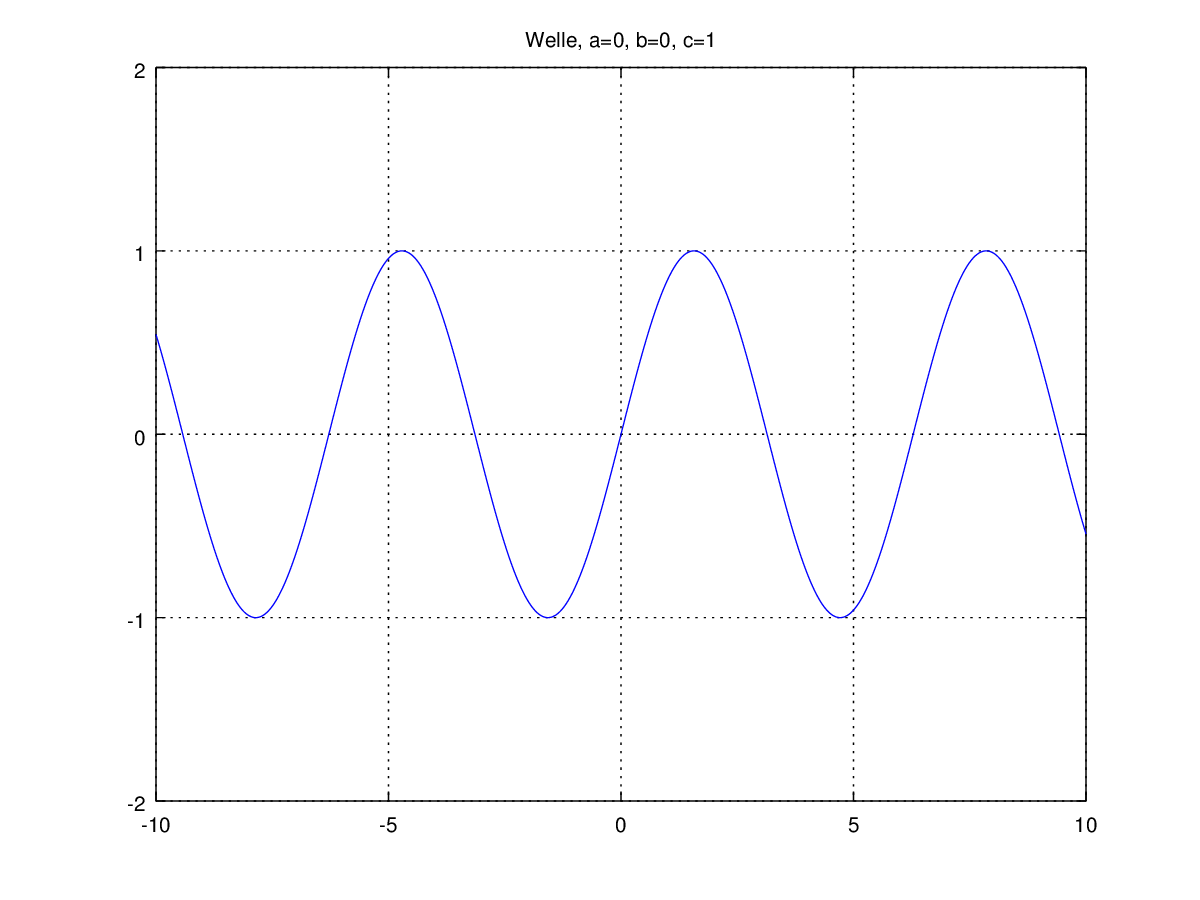
\includegraphics[scale=0.35]{./wellen/images/basicfunctions/sin.png}
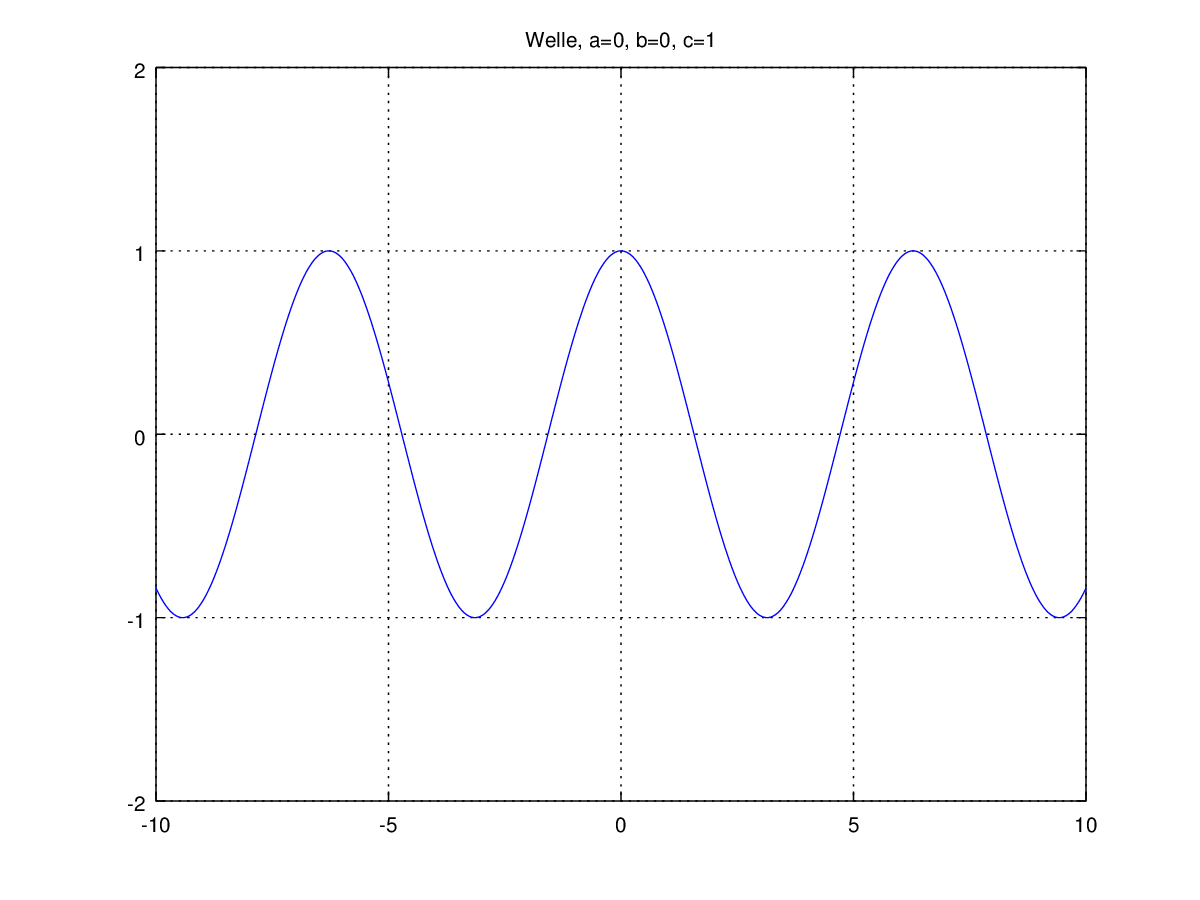
\includegraphics[scale=0.35]{./wellen/images/basicfunctions/cos.png}

F"ur negative Werte von c kann die L"osungsgleichung \ref{wellen:LSGleichung} 
zwar auch verwendet werden, es entstehen aber imagin"are Faktoren durch die 
negativen Wurzelwerten. Die imagin"are Einheit $i$ ist definiert als

\begin{equation}
	i = \sqrt{-1}.
	\label{wellen:imaginaereEinheit}
\end{equation}

Wird dieser Wurzelwert \ref{wellen:imaginaereEinheit} bei jedem negativen Wert 
von $c$ ausgeklammert, ergibt sich die L"osungsgleichung.

\begin{equation}
	\begin{split}
	y(x) &= a_0 \cos(i\sqrt{|c|}x) + \frac{a_1}{i\sqrt{|c|}}\sin(i\sqrt{|c|}x) 
	\\
	\Leftrightarrow
	y(x) &= a_0 \cos(i\sqrt{|c|}x) - i\frac{a_1}{\sqrt{|c|}}\sin(i\sqrt{|c|}x)
	\end{split}	
	\label{wellen:LSGnegcWerte}
\end{equation}

Die Definitionen vom Sinus Hyperbolicus und Cosinus Hyperbolicus lauten:

\begin{equation*}
	\begin{split}
	\sinh(x) &= \frac{1}{2} (e^x - e^{-x}) = -i \sin(ix)\\
	\cosh(x) &= \frac{1}{2} (e^x + e^{-x}) = \cos (ix)
	\end{split}
\end{equation*}

Werden die Definitionen mit der L"osungsformel verglichen, ist ersichtlich, 
dass es sich je nach Wahl von $a_0$ und $a_1$ um eine der beiden hyperbolischen 
Funktionen handelt. Die L"osungsgleichung ergibt sich also zu

\begin{equation}
	y(x) = a_0 \cosh(\sqrt{|c|}x) + \frac{a_1}{\sqrt{|c|}}\sinh(\sqrt{|c|}x)
	\label{wellen:LSGhyperbolFunktion}
\end{equation}

In den folgenden zwei Grafiken wird zuerst der ``reine'' Sinus Hyperbolicus und 
als zweites der ``reine'' Cosinus Hyperbolicus dargestellt.

\noindent
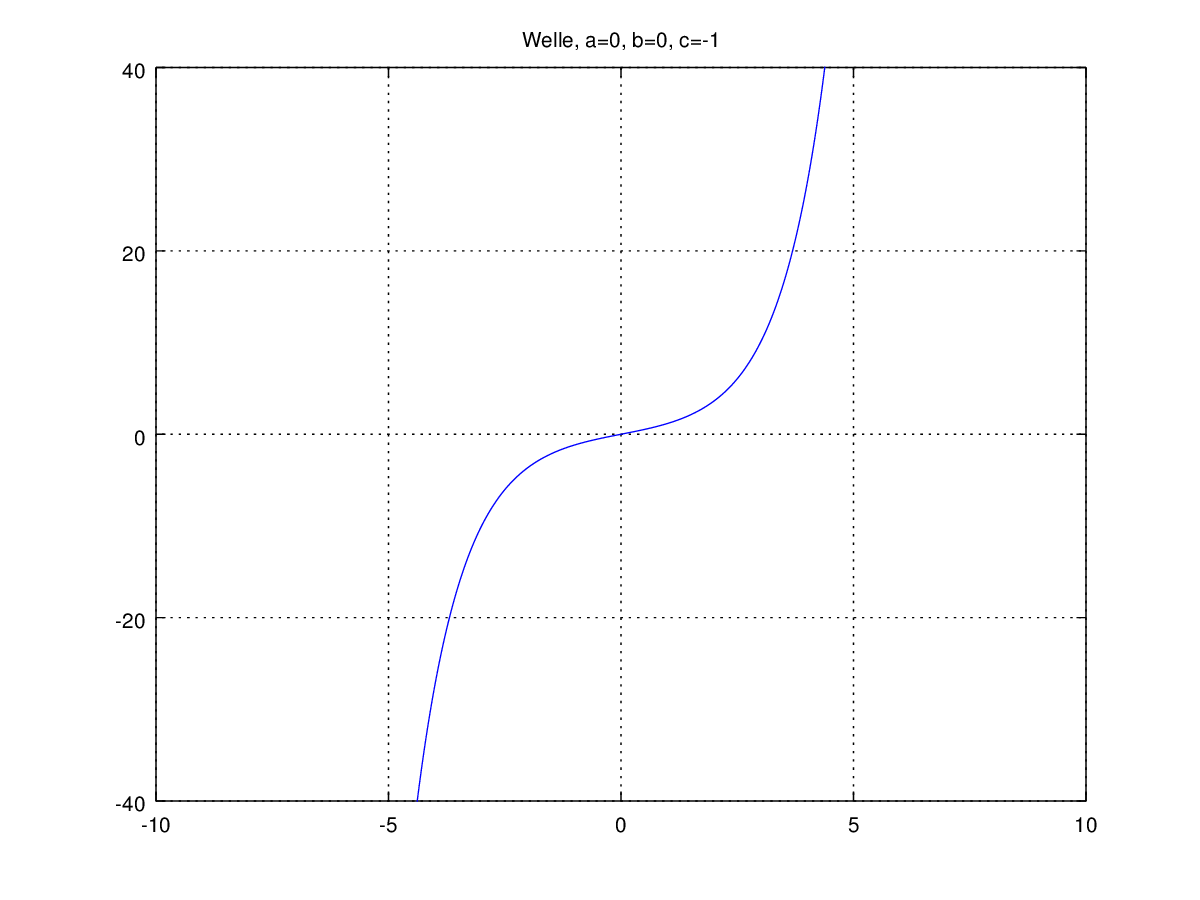
\includegraphics[scale=0.35]{./wellen/images/basicfunctions/sinh.png}
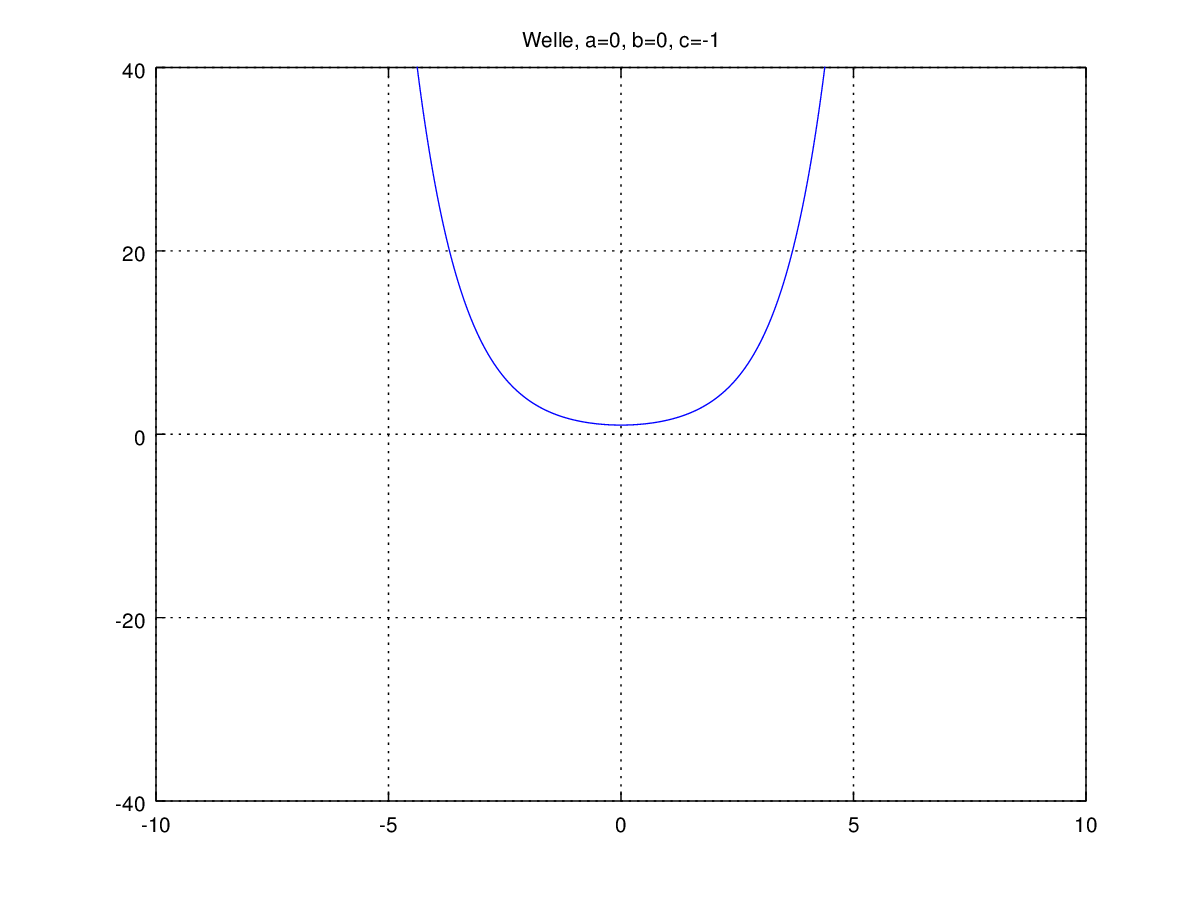
\includegraphics[scale=0.35]{./wellen/images/basicfunctions/cosh.png}

\subsection{Variation von $b$}

Als Zweites werden die Variablen $a$, $c$ und die Anfangsbedingungen 
festgehalten und nur das $b$ ver"andert. Um aufzuzeigen, was sich dabei 
ver"andert, braucht es nur die Parabelgleichung.

\begin{equation*}
	y(x) = ax^2 + bx + c
\end{equation*}

BILD VERSCH. PARABELN

Der Faktor $b$ bezweckt n"amlich, wie man in der Grafik sieht, in der Parabel 
nur eine Verschiebung in Richtung der $x$-Achse. Diese Verschiebung bedeutet in 
der betrachteten Problemstellung nur, dass sich die Schnittpunkte mit der 
$x$-Achse verschieben. Was dies bedeutet wird in einem sp"ateren Abschnitt 
erkl"art. Was aber aus der Variation mit $b$ herausgeht ist, dass wir die 
dadurch ver"anderten Eigenschaften auch mit der Variation von $c$ oder von 
$a_0$ aufzeigen k"onnen. Aus diesem Grund wird die Variabel $b$ in Fortsetzung 
immer gleich 0 gesetzt und damit vernachl"assigt. 

Die neue zu betrachtende Differentialgleichung ergibt sich damit zu:

\begin{equation} 
	y'' + (ax^2 +c)y = 0
	\label{wellen:DGLzubetrachten}
\end{equation}

\subsection{Variation von $c$}
\label{wellen:Variationc}

Als N"achstes wird untersucht, welche Auswirkungen die Variation vom 
Koeffizienten $c$ hat, wenn $a$ vorhanden ist und nicht gegen 0 geht aber 
trotzdem festgehalten wird. $a$ wird in der folgenden Betrachtung gleich 1 
gesetzt.

Der Koeffizient $c$ beschreibt den Schnittpunkt der Parabel mit der $y$-Achse 
und somit die Verschiebung in $y$-Richtung. Diese Verschiebung kann nicht, wie 
die Verschiebung in Richtung der $x$-Achse mit dem Koeffizienten $b$, 
vernachl"assigt werden. Grund daf"ur ist, dass die Wellenform vom Schnittpunkt 
der Parabel mit der $x$-Achse abh"angt. 

\noindent
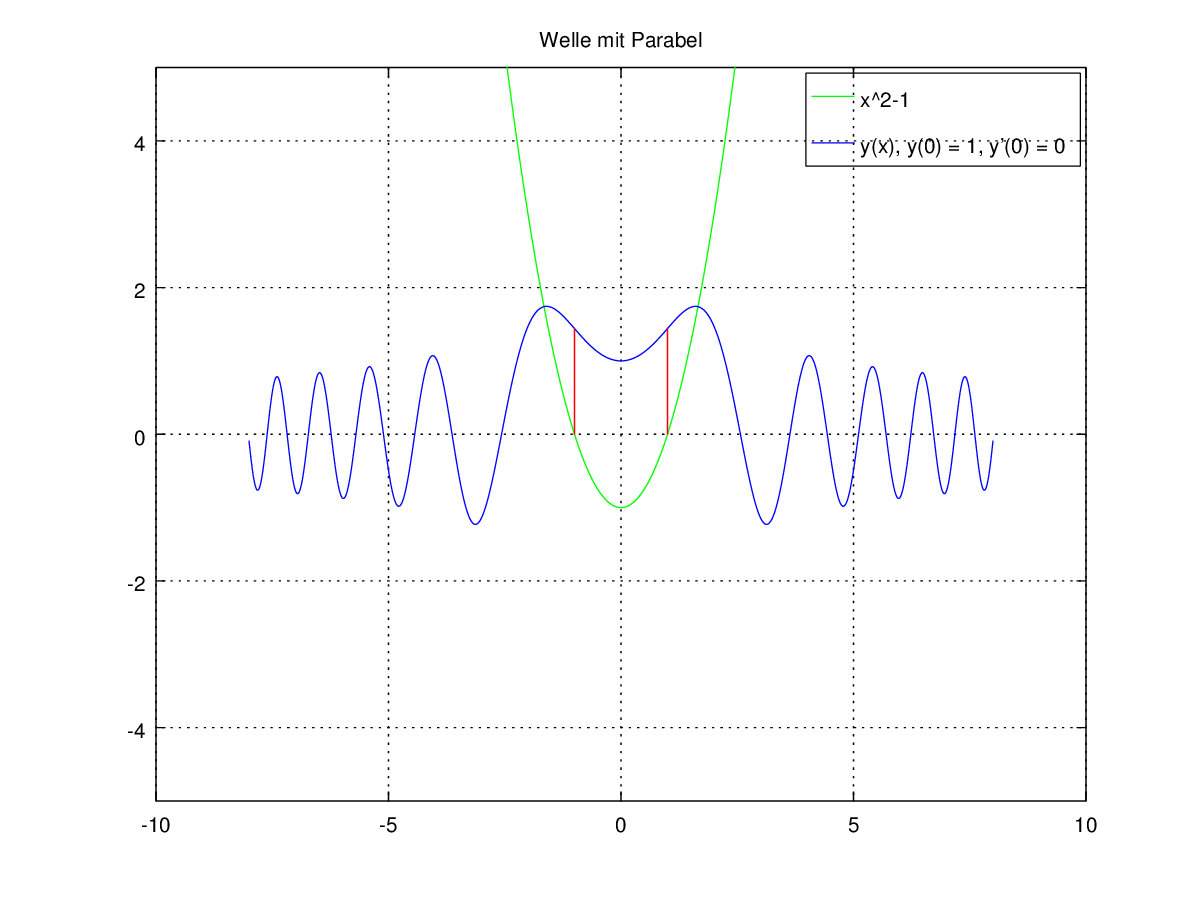
\includegraphics[scale=0.35]{./wellen/images/varc/cneg1.png}
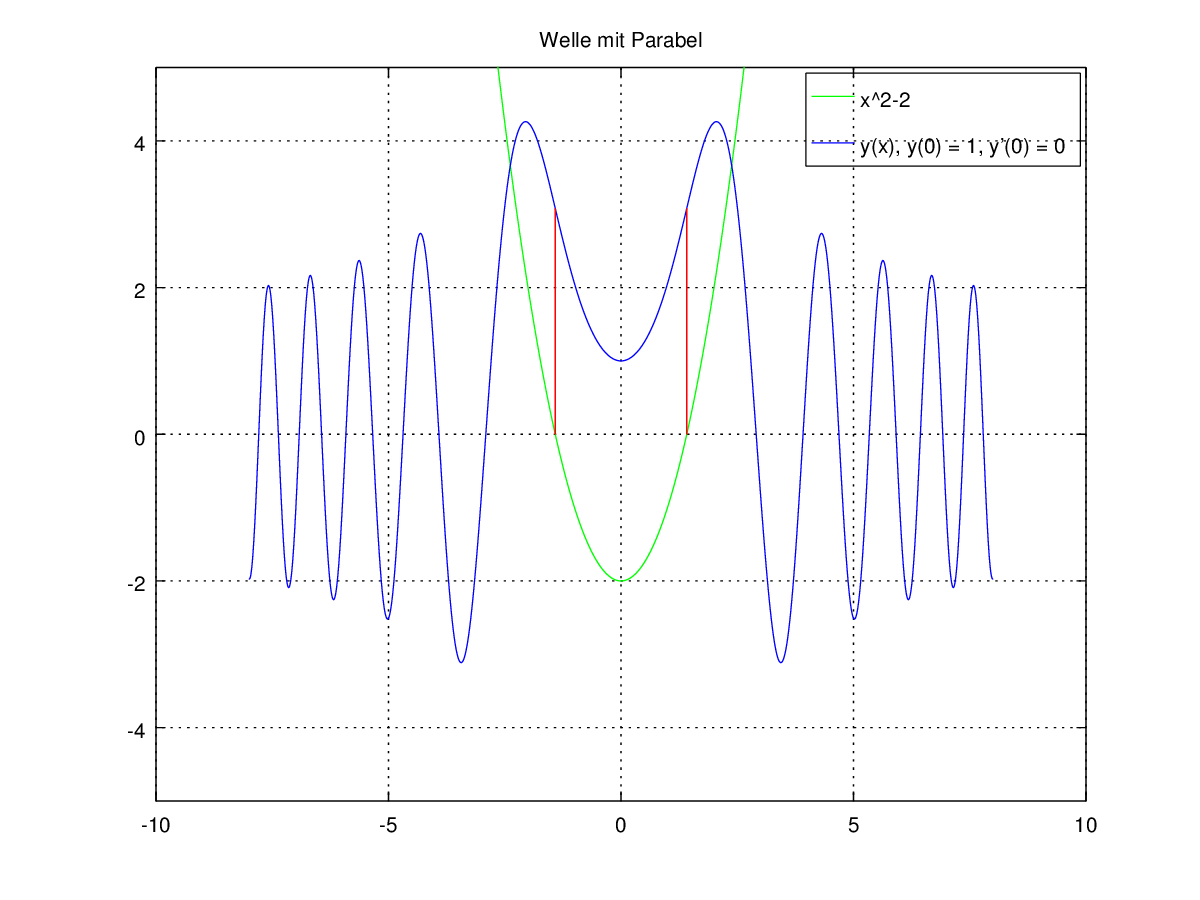
\includegraphics[scale=0.35]{./wellen/images/varc/cneg2.png}

In den zwei Grafiken werden die 
Parabeln mit zwei unterschiedlichen $y$-Achsenabst"anden und deren aus der 
Differentialgleichung \ref{wellen:DGLzubetrachten} entstehende Welle gezeigt. 
Es wird deutlich, dass es nicht die gleiche Welle gibt und dass sich beim 
Schnittpunkt der Parabel mit der $x$-Achse eine "Anderung einstellt. Dieses 
Ph"anomen wird im n"achsten Kapitel \ref{wellen:DiskussionWellenform} erkl"art. 

\subsection{Variation von $a$}
\label{wellen:Variationa}

Zum Schluss wird der Koeffizient $a$ variiert, was zur Folge hat, dass die 
Parabel schl"anker oder enger wird. Dadurch verschiebt sich auch der 
Schnittpunkt der Parabel mit der $x$-Achse und somit auch der Umschlagspunkt, 
der im Kapitel \ref{wellen:Variationc} schon ersichtlich war. 

...

\section{Diskussion der Wellenform}
\label{sec:wellen:DiskussionWellenform}

Wie schon in den vorhergehenden Kapiteln ersichtlich war, wechselt die Welle 
ihre Form im ``Umschlagspunkt'', welcher die Schnittpunkte der Parabel mit der 
$x$-Achse bezeichnet.


Grunds"atzlich gibt sechs untschiedliche F"alle wie die Parabel liegen kann:
\begin{itemize}
	\item Der Schnittpunkt der Parabel mit der $y$-Achse ist im negativen 
	Bereich und die Parabel nach oben ge"offnet
	\item Der Schnittpunkt der Parabel mit der $y$-Achse ist im positiven 
	Bereich und die Parabel ist nach oben ge"offnet
	\item Der Schnittpunkt der Parabel mit der $y$-Achse liegt im Nullpunkt und 
	die Parabel ist nach oben ge"offnet
	\item Der Schnittpunkt der Parabel mit der $y$-Achse ist im negativen 
	Bereich und die Parabel nach unten ge"offnet
	\item Der Schnittpunkt der Parabel mit der $y$-Achse ist im positiven 
	Bereich und die Parabel nach unten ge"offnet
	\item Der Schnittpunkt der Parabel mit der $y$-Achse liegt im Nullpunkt und 
	die Parabel ist nach unten ge"offnet
\end{itemize}

Zu Beginn wird der erste Fall betrachtet, welcher beispielsweise die Parabel 
auf der Grafik im Kapitel \ref{subsec:wellen:Variationc} beschreibt. Diese 
Parabel hat 
zwei Schnittpunkte mit der $x$-Achse und der Scheitelpunkt liegt im negativen 
$y$-Bereich. Dies bedeutet, dass alle L"osungen der Parabel von $x=0$ bis zum 
Schnittpunkt der Parabel mit der $x$-Achse negativ sind. 

Wenn nun in der Differentialgleichung f"ur die Parabel ein beliebiger negativer 
Wert eingesetzt wird, resultiert dieselbe Gleichung 
\ref{eq:wellen:LSGnegcWerte} 
wie im Kapitel \ref{subsec:wellen:Eliminierungab}. Durch das, dass die Parabel 
durch 
einen Wert ersetzt wird, ist die Aufgabenstellung die Gleiche, wie wenn man $a$ 
und $b$ eliminieren und f"ur $c$ einen negativen Wert einsetzen w"urde. In 
diesem Bereich entsteht demzufolge gem"ass Gleichung 
\ref{eq:wellen:LSGhyperbolFunktion} eine hyperbolische Funktion. Welche von den 
zwei hyperbolischen Funktionen entsteht, l"asst sich mit verschiedenen 
Anfangsbedingungen $a_0$ und $a_1$ bestimmen wie man in den folgenden Grafiken 
sieht.

GRAFIK SINH COSH

Beim Schnittpunkt der Parabel mit der $x$-Achse "andert sich das Vorzeichen der 
L"osung der Parabel und es entsteht nicht die Gleichung 
\ref{eq:wellen:LSGnegcWerte} wie oben, sondern die Gleichung 
\ref{eq:wellen:lineareDGL}, welche f"ur positive $c$-Werte aufgestellt wurde. 

Daraus wird ersichtlich, dass sich ab diesem Punkt eine L"osung einstellt, 
welche aus einer "Uberlagerung von $\sin$ und $\cos$ ist. Daraus entsteht die 
regelm"assige, kontinuierliche Schwingung. 


Bei all den anderen F"allen kann das Gleiche beobachtet werden. Bei der Parabel 
die nach oben ge"offnet ist, passiert genau das Umgekehrte. Im Innenbereich der 
Parabel entsteht eine Schwingung und sobald die Parabel die $x$-Achse schneidet 
wandelt sich die Schwingung in eine hyperbolische Funktion um. 4

Bei den Parabeln, die die $x$-Achse im Nullpunkt ber"uhren entsteht nur eine 
Schwingung, respektive nur eine hyperbolische Funktion, je nach Wert von a, 
welcher angibt, ob die Parabel nach oben oder nach unten ge"offnet ist. 
Dasselbe geschieht auch, wenn die Parabel die $x$-Achse gar nicht schneidet. 

\section{Allgemeines Polynom}

\begin{equation}
	y''+\sum_{i=0}^{n}\lambda_ix^i y=0, \quad n \ge 0
	\label{wellen:allgemeinesproblem}
\end{equation}

Aufgrund der bisherigen Beobachtungen ist es nun m"oglich, eine 
allgemein geltende Potenzreihenl"osung f"ur diese Art Differentialgleichungen 
zu erstellen.

Hierzu wird die anf"angliche Parabel $ax^2 + bx + c$ mit dem allgemeinen Polynom

\begin{equation*}
	\lambda_nx^n + \lambda_{n-1}x^{n-1} + \lambda_{n-2}x^{n-2} + \dotsb + 
	\lambda_2x^2 + \lambda_1x + \lambda_0 = \sum_{i=0}^{n}\lambda_ix^i, \quad n 
	\ge 0
\end{equation*}
ersetzt.

Bei der neuen Problemstellung handelt es sich immernoch um eine 
Differentialgleichungen zweiter Ordnung. Es bleibt also eine Abh"angigkeit von 
mindestens zwei zwischen den verschiedenen $a_k$. Zus"atzlich erh"oht sich 
diese jeweils um den Polynomkoeffizientenindex. Daraus folgt nun

\begin{equation*}
	a_k = -\frac{1}{k(k-1)}\sum_{i=0}^{n}a_{k-2-i)}\lambda_i, \quad n \ge 0, 
	a_{k-2-i < 0} =  0.
\end{equation*}
f"ur ein Polynom $n$-ten Grades.

Die Potenzreihenl"osung f"ur \ref{wellen:allgemeinesproblem} lautet somit:
\begin{equation}
	y(x) = a_0 + a_1x - \sum_{k=2}^{\infty}\frac{1}{k(k-1)}\sum_{i=0}^{n}
	\lambda_ia_{k-2-i}x^k, \quad n \ge 0, a_{k < 0} = 0
	\label{wellen:allgemeineloesung}
\end{equation}

\subsection{Schlussfolgerungen}

Mit der Formel \ref{wellen:allgemeineloesung} gibt es nun ein einfaches 
Werkzeug mit dem man allein durch Einsetzen die Potenzreihenl"osung f"ur 
diese Art von Differentialgleichungen erh"alt.

Sie erlaubt es uns aber auch noch weitere Schl"usse zu ziehen. So kann man 
nun direkt aus der Form der L"osung des gegebenen Polynoms ablesen, wie sich 
die Differentialgleichung verhalten wird. Soll heissen, positive L"osungen 
f"uhren zu einer Wellenform, die $\sin$ und $\cos$ enthalten. Negative 
L"osungen liefern hingegen eine Kombination aus $\sinh$ und $\cosh$.

\subsection{Beispiel: $n = 1$, Airy-Differentialgleichung}
Die bereits bekannte Airy-Differentialgleichung
\begin{align*}
	y''-xy = 0
\end{align*}
ergibt nun in die allgemeine L"osungsformel \ref{wellen:allgemeineloesung} 
eingesetzt:

\begin{equation*}
\begin{split}
	y(x) &= a_0+a_1x-\sum_{k=2}^{\infty} \frac{1}{k(k-1)} ((-1) a_{k-2-1} + 0 
	a_{k-2-0}) x^k
	\\
	&= a_0+a_1x+\sum_{k=2}^{\infty} \frac{1}{k(k-1)} a_{k-3} x^k,
	\qquad a_{k < 0} = 0
\end{split}
\end{equation*}

Graphisch betrachtet werden die genannten Konsequenzen deutlich erkennbar:

\begin{center}
	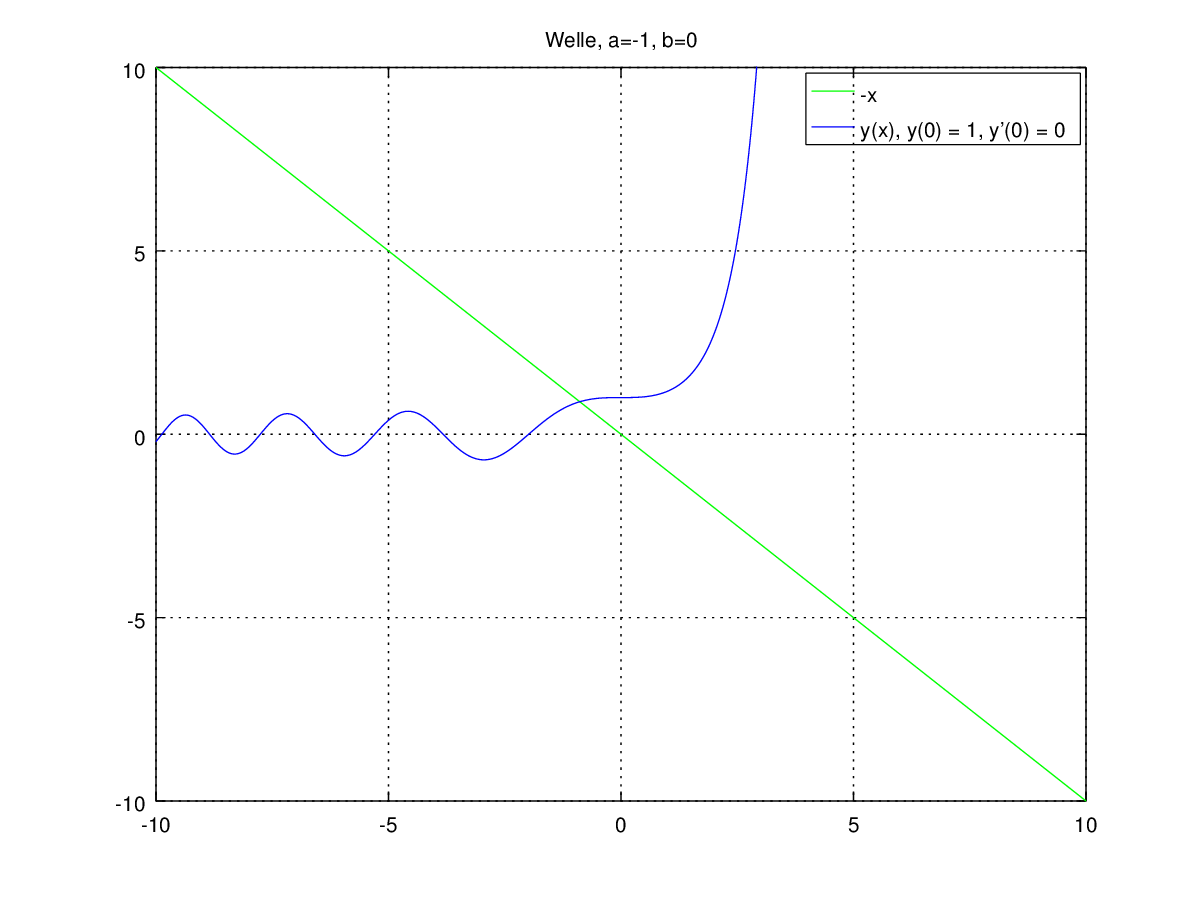
\includegraphics[scale=0.65]{./wellen/images/allgemein/n1.png}
\end{center}

\subsection{Beispiel: $n = 4$}

Auch ein Polynom 4-ten Grades stellt kein Problem dar. Die 
Differentialgleichung:

\begin{equation*}
	y''+(ax^4+bx^3+cx^2+dx+e)y = 0
\end{equation*}
ergibt nach dem Einsetzen:

\begin{align*}
	y(x) &= a_0+a_1x-\sum_{k=2}^{\infty} \frac{1}{k(k-1)} (aa_{k-2-4} + 
	ba_{k-2-3} + ca_{k-2-2} + da_{k-2-1} +ea_{k-2-0})x^k
	\\
	&= a_0+a_1x-\sum_{k=2}^{\infty} \frac{1}{k(k-1)} (aa_{k-6} + ba_{k-5} + 
	ca_{k-4} + da_{k-3} +ea_{k-2})x^k, \qquad a_{k<0} = 0
\end{align*}

Auch hier kann man graphisch die "Uberg"ange zwischen $\sin$ und $\cos$ bei 
positiven und $\sinh$ und $\cosh$ bei negativen Polynoml"osungen klar erkennen.

\begin{center}
	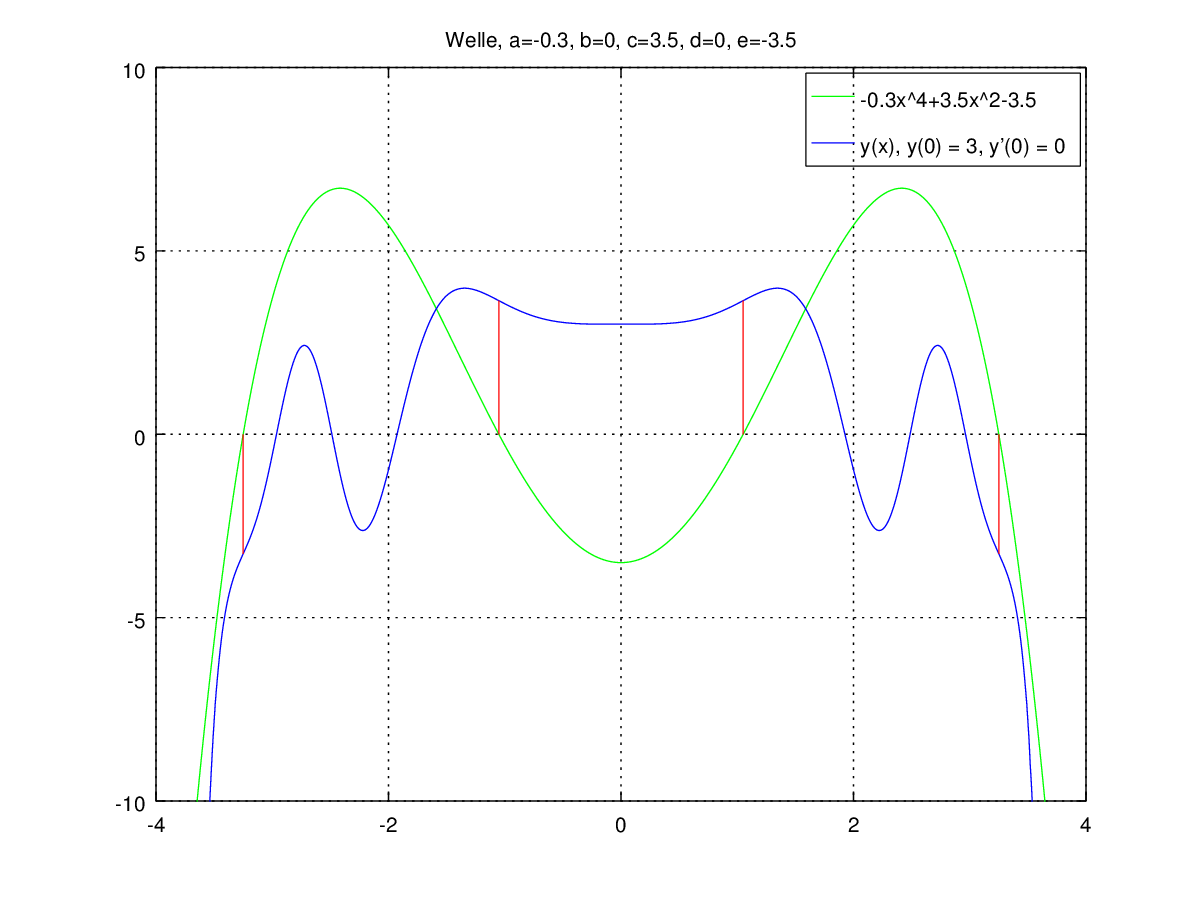
\includegraphics[scale=0.65]{./wellen/images/allgemein/n4.png}
\end{center}


\printbibliography[heading=subbibliography]
\end{refsection}